\documentclass[../../document.tex]{subfiles}
\begin{document}

\section*{Aufgabe 1}

\subsection*{a)}

\subsubsection*{1.)}

\begin{figure}[H]
    \begin{center}
        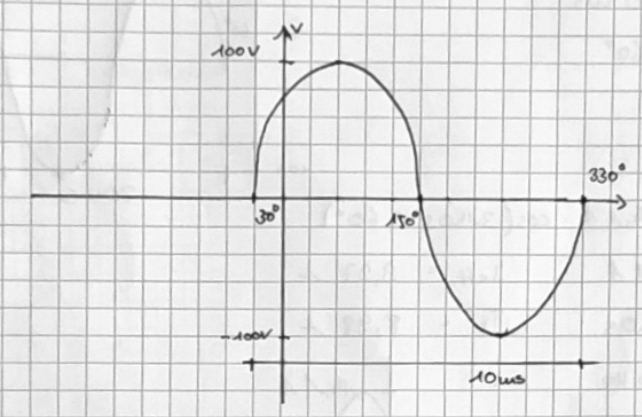
\includegraphics[width=.9\linewidth]{../../img/aufg1-a-1}
    \end{center}
\end{figure}

\begin{equation*}
    \begin{split}
        u(t) &= \SI{100}{\volt} * \cos(\SI{628}{\second} * t + \SI{30}{\degree})\\\\
        \hat{u} &= \SI{100}{\volt} &\rightarrow &  Spitzenwert\\
        T &= \frac{1}{f} \approx \SI{10}{ms} &\rightarrow &  Periodendauer\\
        \omega &= \SI{628}{\second} &\rightarrow &  Kreisfrequenz\\
        f &= \frac{\SI{628}{\second}}{2\pi} = \SI{99,95}{\hertz} &\rightarrow &  Frequenz\\
        u\cind{eff} &= \frac{\hat{u}}{\sqrt{2}} = \SI{70,71}{\volt}\\
        \left\lvert\bar{u}\right\rvert &= \frac{2 * \hat{u}}{\pi} = \SI{63,66}{\volt}\\ 
        \bar{u} &= 0\\
        \varphi &= \SI{30}{\degree}\\
    \end{split}
\end{equation*}

\newpage

\subsubsection*{2.)}

\begin{figure}[H]
    \begin{center}
        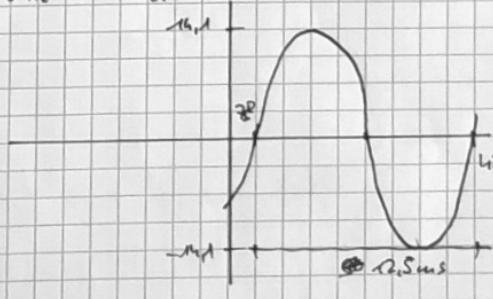
\includegraphics[width=.9\linewidth]{../../img/aufg1-a-2}
    \end{center}
\end{figure}

\begin{equation*}
    \begin{split}
        u(t) &= \SI{14,4}{\volt} * \cos(\SI{503}{\second} * t - \SI{75}{\degree})\\\\
        \hat{u} &= \SI{14,4}{\volt}\\
        u\cind{eff} &= \SI{9,97}{\volt}\\
        \left\lvert\bar{u}\right\rvert &= \SI{8,98}{\volt}\\
        \bar{u} &= 0\\
        T &= \frac{1}{\SI{80}{\hertz}} = \SI{12,5}{ms}\\
        f &= \frac{\SI{503}{\second}}{2\pi} = \SI{80,05}{\hertz}\\
        \omega &= \SI{503}{\second}\\
        \varphi &= \SI{75}{\degree}\\
    \end{split}
\end{equation*}

\newpage

\subsubsection*{3.)}

\begin{figure}[H]
    \begin{center}
        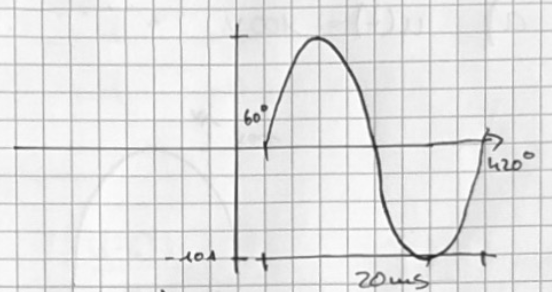
\includegraphics[width=.9\linewidth]{../../img/aufg1-a-3}
    \end{center}
\end{figure}

\begin{equation*}
    \begin{split}
        i(t) &= \SI{10}{\ampere} * \cos(\SI{3140}{\second} * t - \SI{60}{\degree})\\
        \hat{I} &= \SI{14,4}{\ampere}\\
        I\cind{eff} &= \SI{9,97}{\ampere}\\
        \left\lvert\bar{I}\right\rvert &= \SI{8,98}{\ampere}\\
        \bar{I} &= 0\\
        \omega &= \SI{3140}{\second}\\
        f &= \SI{500}{\hertz}\\
        T &= \SI{2}{ms}\\
        \varphi &= \SI{60}{\degree}\\
    \end{split}
\end{equation*}

\newpage

\subsubsection*{4.)}

\begin{figure}[H]
    \begin{center}
        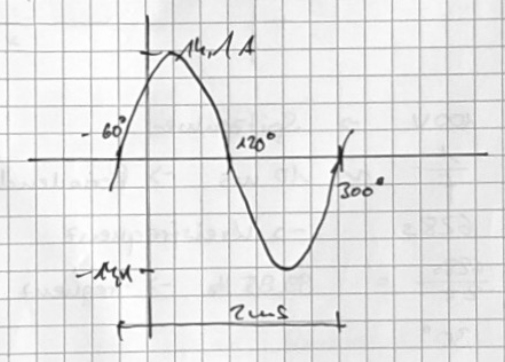
\includegraphics[width=.9\linewidth]{../../img/aufg1-a-4}
    \end{center}
\end{figure}

\begin{equation*}
    \begin{split}
        i(t) &= \SI{14,4}{\ampere} * \cos(\SI{3140}{\second} * t + \SI{60}{\degree})\\
        \hat{I} &= \SI{14,4}{\ampere}\\
        I\cind{eff} &= \SI{9,97}{\ampere}\\
        \left\lvert\bar{I}\right\rvert &= \SI{8,98}{\ampere}\\
        \bar{I} &= 0\\
        \omega &= \SI{3140}{\second}\\
        f &= \SI{500}{\hertz}\\
        T &= \SI{2}{ms}\\
        \varphi &= \SI{60}{\degree}\\
    \end{split}
\end{equation*}

\newpage

\subsection*{b)}

Über das Integral wird die Fläche zwischen der Funktion und der x-Achse des Graphen bestimmt. 
Dies ist der Flächeninhalt der Funktion im Integrationsbereich.

\subsection*{c)}

\textbf{Effektivwert}

\begin{itemize}
    \item quadratischer Mittelwert der Funktion
    \item durch Quadrierung: immer positiv
    \item am Ende: Wurzel ziehen
\end{itemize}

\textbf{Gleichrichtwert}

Hier wird für der Mittelwert des Betrags betrachtet

\textbf{Mittelwert}

\begin{itemize}
    \item bei einer Sinusform, wie hier im Beispiel: 0
    \item zu gleichen Teilen oberhalb und unterhalb der x-Achse
\end{itemize}

\subsection*{d)}

\textbf{RMS-Leistung - Root Mean Square}

\begin{itemize}
    \item Englisch für quadratisches Mittel: Effektivwert
    \item amtliche richtige Aussage über Leistung von z.B. Lautsprechern
\end{itemize}

\subsection*{e)}

\textbf{Periodische Funktion}

Regelmäßige Widerholung von Funktionswert in wiederkehren "Perioden"

\subsection*{f)}

\textbf{3 Beispiele}

\begin{itemize}
    \item Ideale Feder mit Gewicht
    \item Sinusfunktion
    \item Riesenrad
\end{itemize}

\subsection*{g)}

\begin{itemize}
    \item Drehstromnetz
    \item Nachrichtenübertragung
    \item Regelungstechnik
\end{itemize}

\end{document}